\subsection{SHAP Evidence and Software-Module Suspect Ranking}
\label{sec:shap_module_results}

This experiment asks whether predicted-class TreeSHAP contributions can be organized into conserved and prediction-relevant telemetry evidence, and whether commit-specific uORB propagation provides useful software-module inspection candidates. The primary explanation analysis was ground-truth-anomaly-conditioned: it used all 3602 labelled anomalous test windows from the fixed chronological protocol and did not require Stage 1 to detect them. For each window, the TreeSHAP contributions of the predicted Stage 2 class were converted to absolute evidence and aggregated from statistical features to telemetry channels, PX4 topics, and subsystems. The aggregation preserved the total evidence mass: the maximum absolute conservation error across the hierarchy was $7.11 \times 10^{-15}$. This verifies only the numerical redistribution of evidence; it does not establish that the attributed channel or subsystem is the physical source of the anomaly.

The masking analysis tested whether the validation-derived SHAP ranking was more informative than an equal-size random feature selection. The top-$k$ SHAP features were ranked on validation anomaly windows and replaced in the test data by feature-wise medians calculated from the training windows. The Macro-F1 decrease for SHAP masking increased from 0.0409 at $k=10$ to 0.2683 at $k=100$. Across 20 random subsets nested within each of five model seeds, the paired SHAP-minus-random advantage was 0.0404 (95\% flight-log-bootstrap CI [0.0102, 0.0713]) at $k=10$ and 0.2646 [0.2052, 0.3300] at $k=100$. Replacing the selected feature block with values from sampled training rows produced drops of 0.0516 [0.0277, 0.0752] and 0.4955 [0.4604, 0.5283], respectively. The direction therefore persisted under both median and joint-donor perturbations, although donor replacement can still create cross-block combinations with unreplaced features. These results support prediction-relevant feature concentration, not causal influence or physical necessity.

At the telemetry-channel level, agreement depends on the semantic reference. Under the document-derived mapping, overall Consistency@1 was $0.2500\pm0.0056$, compared with the exact random baseline of 0.1707. External Position remained near random and Global Position below random; therefore, the positive masking result is evidence of prediction relevance, not uniform agreement with physical fault domains. Supplementary Material Section S2 reports the complete class-level results and the 11 changed channel assignments.

For the architecture-aware layer, the unfiltered static scan at commit \texttt{\seqsplit{82aa24adfca29321cfd1209e287eab6c2b16780e}} contained 180 topic-role-module edges covering 54 PX4 modules. The 244-occurrence internal consistency check returned 1.000 agreement and edge recovery within its shared-vocabulary scope; it is not an independent uORB gold audit. Conservative source-path exclusion removed 35 edges and 18 modules, leaving 145 edges, 36 modules, and all 18 topics while preserving evidence conservation. Producer Top-3 overlap was 3/3 before versus after filtering, while Top-5 overlap was 4/5; bidirectional Top-5 was unchanged. Under filtered producer-only propagation, the highest-ranked source-tree inspection candidates were \path{src/modules/mavlink} (SHAP share 0.2572), \path{src/modules/ekf2} (0.2318), \path{src/modules/sensors} (0.1243), \path{src/modules/vtol_att_control} (0.0811), and \path{src/modules/position_estimator_inav} (0.0708). Figure~\ref{fig:shap_module_evidence}(b) shows this conservative-exclusion result. The exclusion is path-based and does not reconstruct the compiled PX4FMU\_V2 build; degree normalization and propagation-mode sensitivity further preclude interpreting the order as a stable root-cause ranking.

The separate Stage-1-gated matching-commit analysis used the frozen validation-derived detector thresholds. Averaged across the five seeds, the 14,419 matching-commit test windows comprised 937.2 true positives, 455.8 false negatives, 532.2 false positives, and 12,493.8 true negatives; mean detector recall was $0.6728 \pm 0.0248$ and precision was $0.6398 \pm 0.0305$. Thus, only the true-positive subset can carry detected real-anomaly evidence downstream, while the false-negative subset is absent from a deployed gate. The false-positive windows were assigned by Stage 2 to External Position (128.8), Global Position (216.4), Altitude (88.4), and Mechanical/Electrical (98.6) on average. These are predicted suspect categories for false alarms, not validated fault labels. This gated analysis is reported separately from the 1393-window ground-truth-anomaly-conditioned analysis.

Figure~\ref{fig:shap_module_evidence} summarizes the masking comparison and conservatively filtered commit-level source-tree candidates. Selected frozen analysis records are described in the Data Availability Statement.

\begin{figure}[H]
    \centering
    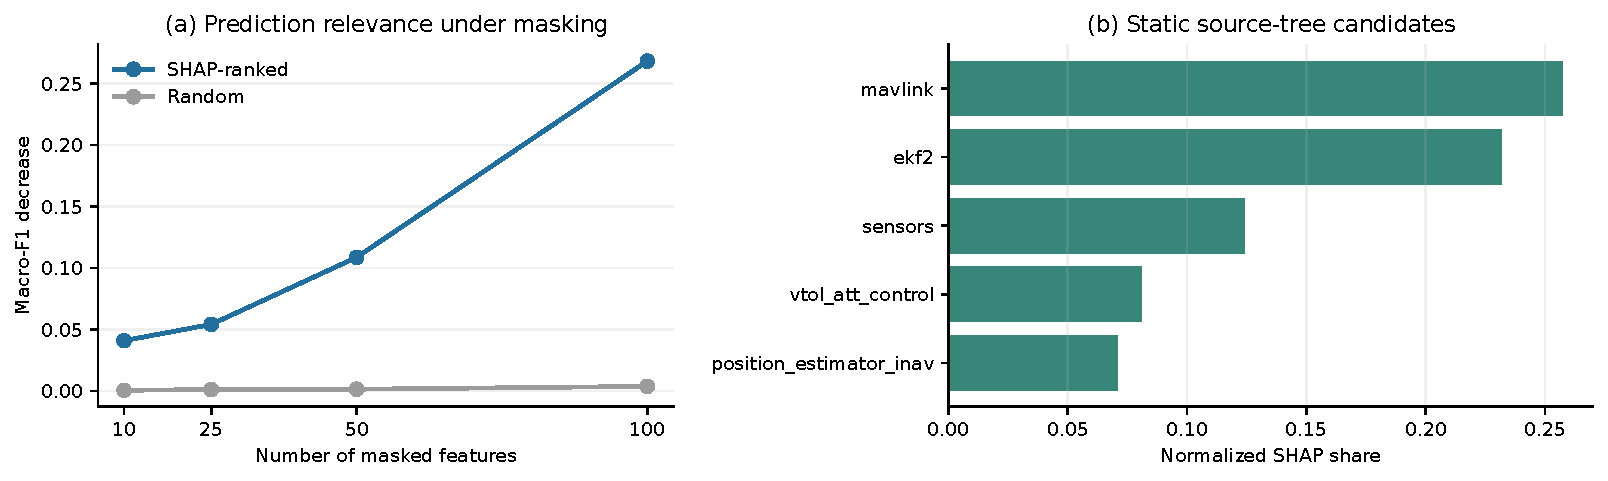
\includegraphics[width=\textwidth]{figures/figure_4_evidence_revision.pdf}
    \caption{Prediction-relevant evidence and architecture-aware candidates. (a) Mean Macro-F1 decrease after masking validation-ranked SHAP features or equal-size random subsets; uncertainty for paired contrasts is reported in the text, rather than mixing seed variation with random-mask repetitions. (b) Filtered producer-only source-tree candidates from the 1393 ground-truth anomalous test windows whose firmware matches the selected commit; bars are mean normalized shares across seeds. These aggregate real-flight candidates are not mutation-trial localization scores. Complete semantic-map sensitivity is retained in Supplementary Material Section S2.}
    \label{fig:shap_module_evidence}
\end{figure}
